\chapter{Interpolation af funktioner}
% God arbejdslyst
% 
%%%%%%%%% INTRODUKTION %%%%%%%%%
%
\begin{color}{AAUblue2}
Dette dokument giver en grundlæggende forståelse for Lagrange interpolation samt numerisk integrering. 
%
\end{color}
\\\\
%
%%%%%%%%%%% OPGAVE 1 %%%%%%%%%%%
\section*{1. Lagrange interpolation}
%
\begin{color}{AAUblue2} Gennemgå teorien for Lagrange interpolation baseret på datapunkterne $x_0, \ldots, x_N$ og $f_0, f_1, \ldots , f_N$. 
\end{color}
\\\\ 
%
Lagrange interpolation handler om at finde et polynomium $p(x_k)=f(x_k)$ og er således en måde at approksimere en funktionsværdi givet $x_0 \ldots x_N$ og $N+1 $  $y$ værdier.
Det ønskes således at finde et polynomium med interpolationsegenskaben $p_{x_j}=y_j$,$j=0,1,\ldots,N$.

Problemet omhandler således at finde et $N$'te grads polynomium $p$, der tager funktionsværdien for $f$ i en givet mængde punkter. 
Ideen kan således relateres til taylorserier og konstruktion af taylorpolynomier, da disse ligeledes antager funktionsværdien i et givet udviklingspunkt.
Lagrange polynomier er defineret ved:
\begin{align*}
l_k(x)=\frac{\prod_{\substack{j=0 \\ {j \neq k}}}^{N}(x-x_j)}{\prod_{\substack{j=0 \\ {j \neq k}}}^{N}(x_k-x_j)}=\frac{(x-x_0) \cdots (x-x_{j-1}) \cdot (x-x_{j+1})\cdots(x-x_N)}{(x_j-x_0)\cdots (x_j-x_{j-1}) \cdot (x_j-x_{j+1})\cdots (x_j - x_N)}
\end{align*}
og et Lagrange-interpolerede andensgradspolynumium er således givet ved:
\begin{align*}
p(x)=f(x_0)\frac{(x-x_1)(x-x_2)}{(x_0-x_1)}+f(x_1)\frac{(x-x_0)(x-x_2)}{(x_1-x_0)(x_1-x_2)}+f(x_2)\frac{(x-x_0)(x-x_1)}{(x_2-x_0)(x_2-x_1)}
\end{align*}
Der eksisterer et entydigt Lagrange interpoleret polynomium for punkter givet ved $x_0, \ldots, x_N$ og $f_0, f_1, \ldots , f_N$.
\\\\
% 
\begin{proof}
Ved at finde sådanne polynomier, er deres eksistens bevist. Deres entydighed vil nu bevises. 
Antag, at $q_n$ og $p_n$ er to forskellige polynomier med grad $\leq n$, og at de begge interpolerer samme data. 
Så er graden af polynomiet $p_n - q_n$ også $\leq n$, og værdien af dette polynomie er $0$ ved $n+1$ datapunkter. 
Men en polynomie med grad $n$ har højst $n$ nuller, medmindre det er nulpolynomiet. 
Således er $p_n - q_n = 0$, hvormed $p_n = q_n$. 
\end{proof}
%
%%%%%%%%%%% OPGAVE 2 %%%%%%%%%%%    
\section*{2. Definition af funktion}
%
\begin{color}{AAUblue2} 
Vi definerer funktionen $f$ ved
\begin{align*}
f(x)=x^2-\sin(10x), x \in \mathbb{R}
\end{align*}
Vi ser på intervallet $\left [0,3 \right ]$ og definerer punkterne $x_j = \frac{3j}{N}, j = 0, 1, \ldots, N$, så at vi har $N+1$ ækvidistante punkter. Vi definerer også $f_j=f(x_j), j=0,1,\ldots,N.$ Vi betegner med $p_N$ det interpolerende polynomium baseret på disse data.  
\end{color}
%
%%%%%%%%%%% OPGAVE 3 %%%%%%%%%%%
\section*{3. }
%
\begin{color}{AAUblue2} 
Scriptet \textsc{Interpolation bin.py} giver en vurdering af den maksimale fejl 
\begin{align*}
\underset{x \in \left [0,3 \right ]}{\text{max}} \lvert f(x)-p_N(x) \rvert
\end{align*}
for forskellige værdier af $N$. Det beregner også en teoretisk vurdering af fejlen, se nedenfor. Gennemgå dette script i detaljer. \textbf{Bemærk} at dette script ikke bruger \textsc{numpy}, men er baseret på lister. Begrundelsen er at vi skal være i stand til at modificere dette script til at anvende \textsc{decimal modulet}. Efter gennemgangen skal I modificere scriptet til at generere plots for små værdier af $N$, der i samme figur viser grafen for $f(x)$, grafen for $p(x)$ og knudepunkterne.
% 
\end{color}
\\\\ 
%
I scriptet starter man med at definere Lagrange funktionen. Dette gøres ved hjælp af lister, og en for-løkke, hvor j ikke må være lig k. Den ganger resultaterne fra listen temp sammen, og finder produktet.

Så findes Lagrange interpolation polynomium. Så opskrives parametrene og funktioenn der ønskes undersøgt. Programmet finder efterfølgende nogle x- og y-værdier samt afstanden mellem x-værdierne. Så udregner programmet approximationen og løsningen. Til sidst udregner programmet fejlen og printer noget data. 

I python scriptet \textsc{Interpolation bin funktioner.py}, ses modificeringen, så den generer plots for små værdier af N, som i samme figur viser grafen for $f(x)$, grafen for $p(x)$ og knudepunkterne. 
%
%\subsubsection*{Python script}
%
%\lstset{style=mystyle}
%\lstinputlisting[language=Python]{code/funktion.py}
%
%
%Obs. spørg ind til hvorfra "Error bound" delen opstår (linje 31-34), og hvordan man kommer frem til dette 
%
%%%%%%%%%%% OPGAVE 4 %%%%%%%%%%%
\section*{4. Grafisk undersøgelse}
%
\begin{color}{AAUblue2} 
Lav en grafisk undersøgelse af fejlen $\lvert f(x)-p_N(x) \rvert$, for en række forskellige værdier af N baseret på en modificeret udgave af \textsc{Interpolation bin.py.}
\end{color}
\\\\
Man kan se, at approximationen passer til funktionen, når N = 15,30 og 45. Hvis der indsættes andre værdier, eksempelvis 16, 31 og 46 kan der ses, at der opstår store udsving i yderpunkterne i definitionsmængden [0,3], hvilket også stemmer overens med forlæsningsnoterne fra kursusgang 5(s.4-5) hvor der kan ses, at Runge har bevist, at yderpunkterne divergerer.
%
\begin{figure}[h!]
\begin{center}
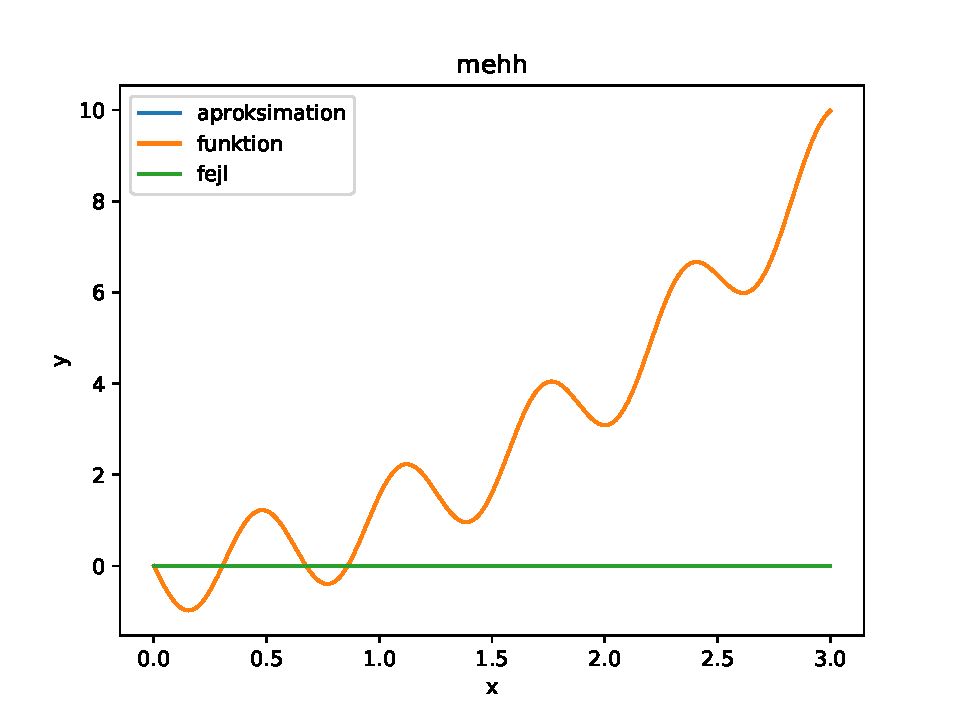
\includegraphics[scale=0.9]{code/del2}
\end{center}
\caption{Fisk.}
%
\end{figure} 
%%%%%%%%%%% OPGAVE 5 %%%%%%%%%%%
\section*{5. Teoretisk vurdering af fejlen}
%
\begin{color}{AAUblue2} 
Brug Theorem 16 i afsnit 6.2 i Turner til at lave en teoretisk vurdering af fejlen
\begin{align*}
\underset{x \in \left [0,3 \right ]}{\text{max}} \lvert f(x)-p_N(x) \rvert.
\end{align*}
%% SE HJÆLP I OPGAVEFORMULERING %% JA TAK %%
%
%%%%% THEREOM 16 %&%%%%
\begin{align*}
f(x)-p(x) = \frac{(x-x_0)(x-x_1)\cdots(x-x_N)}{(N+1)!}f^{(N+1)}(\xi)
\end{align*}
\text{for ethvert} $\xi$ $\in$ $\left [a,b \right ]$.
%%%%%%%%%%%%%%%%%%%%%%%
\\
%%%%% HINT 1/2 %&%%%%
Lad
\begin{align*}
L(x)=(x-x_0)(x-x_1)\cdots(x-x_N).
\end{align*}
%%%%%%%%%%%%%%%%%%%%%%%
\\
For ækvidistante punkter $x_{j+1} - x_j = h$ kan man vise, at der gælder
%%%%% HINT 2/2 %&%%%%
\begin{align*}
\lvert L(x) \rvert \leq \frac{1}{4}(N+1)!h^{N+1}, \text{   } x \in \left [x_0, x_N \right ].
\end{align*}
%%%%%%%%%%%%%%%%%%%%%%%
\end{color}
\\
%
Udtrykket for maksimal fejl kan derfor omskrives til
\begin{align*}
\underset{x \in \left [0,3 \right ]}{\text{max}} \lvert f(x)-p_N(x) \rvert \leq \frac{{1}{4}(N+1)!h^{N+1}}{(N+1)!}f^{(N+1)}(\xi)=\frac{1}{4}h^{N+1}f^{(N+1)}(\xi).
\end{align*}
Det skal nu vises at denne er lig  $0.25h^{(N+1)}M$ for $M=10^{(N+1)}$ ved funktionen $f(x)=x^2-\sin(10x), x \in \mathbb{R}$ i intervallet $a=0$ til $b=3$, hvor $h$ er antallet af steplings, bliver $h=abs(b-a)/N$. 
Det skal nu vises at $f(x)^{(N+1)}(\xi)$ kan omskrives til $M=10^{(N+1)}$
for $N=0$ gælder: $f'(x)=2x-10cos(10x)$ for $n=1$ gælder at $f''(x)=2+100sin(10x)$ for $n=2$ gælder $f'''(x)=1000sin(10x)$ den afledede vil herefter skifte mellem sinus og cosinus og maksimalværdien for disse vil altid være 1 og den maksismale værdi for N'te afledte bliver derfor $10^{N+1}$.
\\
%%%%%%%%%%% OPGAVE 6 %%%%%%%%%%%
\section*{6. Størrelsen af N}
%
\begin{color}{AAUblue2} 
Hvor stor skal $N$ være, for at fejlen er mindre end $10^{-10}$? 
Brug den oprindelige version af \textsc{Interpolation bin.py} til at sammenligne teori og numerisk eksperiment. 
Hvad er konklusionen? 
Hvor kommer problemerne fra? 
I den forbindelse kan I inddrage den grafiske undersøgelse fra punkt 4.
\\
\end{color}
\\
%
Den teoretiske fejl (max) bliver $10^{-10}$ ved $N=48$, men i det numeriske eksperiment bliver fejlen aldrig mindre eller lig $10^{-10}$. Det problematiske er divergens i yderpunkterne, hvilket gør fejlen betydeligt større end den teoretiske, da de går mod $ \infty $ og $ - \infty $. Disse divergenspunkter kan også ses på grafen af $f(x)$ og $p(x)$. 
%
%%%%%%%%%%% OPGAVE 7 %%%%%%%%%%%
\section*{7. Sammenligning af fejlen}
%
\begin{color}{AAUblue2} 
Gentag undersøgelserne af den maksimale fejl og sammenlign med den teoretiske vurdering ved at bruge decimalaritmetik-scriptet \textsc{Interpolation dec.py}. 
Prøv med forskellige værdier for antallet af betydende cifre. 
Hvad er konklusionen?
\\
\end{color}
\\
%
Ved lave værdier af betydende cifre er der dårlig præcision, og fejlen overstiger det teoretiske øvre estimat for grænsen. 
Vælges derimod et højt antal betydende cifre, eksempelvis $80$, bliver computationstiden højere, men fejlen forbliver mindre end grænsen for alle værdier af $N$.
Dette sker da der ved tidligere afrundinger skabes en situation, hvori afrundringsfejlen bliver mere problematisk des højere værdi af $N$ idet der multipliceres med afrundingsfejl i flere iterationer.
%%%%%%%%%%% OPGAVE 8 %%%%%%%%%%%
\section*{8. Chebyshevpunkterne}
%
\begin{color}{AAUblue2} 
Vi erstatter nu de ækvidistante punkter $x_j , j = 0, 1, \ldots , N$ med Chebyshevpunkterne $\Tilde{x}_j = 3 \frac{(1 -\cos(\frac{j \pi}{N}))}{2}, j = 0, 1, \ldots , N$. 
Gennemfør den grafiske undersøgelse fra punkt 4. ovenfor med dette valg af knudepunkter. 
Hvad kan man konkludere ud fra denne undersøgelse?
\\
\end{color}
\\
%
Ved valg af Chebyshevpunkterne som x-værdier sker der ikke de store udsving omkring grænseværdierne, og der ses tendens til at fejlen stablieres omkring $10^-{-14}$ ved $N=40$ og frem. 
Der er dog små udsving i værdien herefter og ikke et entydigt mønster i, hvorvidt aproksimationen bliver bedre.
At aproksimationen stabliseres omkring yderpunkterne er endvidere i overenstemmelse med teorien, hvor disse netop er karakteriseret ved at minimere Runges fænomen.
%%%%%%%%% DONZO GONZO %%%%%%%%%%
% Har vi overvejet nr 9? 
